\documentclass[a5paper,twoside,openany]{book}
\usepackage[body={12cm,18cm}]{geometry}
\usepackage[a5,center,off]{crop}
\usepackage{titlesec}  % For customizing title formats
\usepackage{enumitem}
\usepackage{caption}
\pagestyle{plain}
\usepackage{graphicx}
\usepackage{wrapfig}
\usepackage{lipsum}
\usepackage{kantlipsum}
\usepackage{enumitem}
\graphicspath{ {./images/} }

\newenvironment{normalize}{\leftskip-\leftmargin}{\par}

\begin{document}


\setlength\parindent{0pt}

\titleformat{\chapter}[block]
  {\normalfont\huge\bfseries\centering} % Format for chapter title: huge font, bold
  {\thechapter} % Include the chapter number (e.g., "1")
  {1em} % Spacing between the chapter number and the title
  {} % Text before the chapter title (e.g., "Chapter 1 Title")

% Reducing title and section spacing  
\titlespacing*{\chapter} {0pt}{0ex}{0ex}

% Customizing the Table of Contents title
\renewcommand{\contentsname}{\small Sumario}
\renewcommand{\chaptername}{\small Capítulo}

% Title Page (optional)
\title{%
	Guía para aprender a reparar tus propios aparatos electrodomésticos y electrónicos\\
	\small (¡incluso si nunca has cogido un destornillador!)
	}

\author{%
	David M. \\
	\small Asociación \\ 
	"l'Ateliéphémère"  \\\\
	Traducción: RestartersVLC \\
	}

\maketitle

\tableofcontents
\newpage
 

% Example content
\chapter{Introducción}
\section{Presentación de L'ateliéphémère}

L'ateliéphémère es una asociación que ofrece talleres (así como cursos de formación sobre
sobre temas específicos) para ayudarte a aprender a reparar tus propios
equipos eléctricos y electrónicos, electrodomésticos, etc.\\

\textbf{\underline{¿Cómo funciona?}}

Alguien trae su electrodoméstico averiado, explica el problema y juntos intentamos repararlo.

Pero como siempre aprendemos mejor haciéndolo nosotros mismos, es la persona que ha traído
la persona que ha traído el aparato utilizará las herramientas disponibles in situ.
herramientas.

El objetivo de estos talleres es demostrarnos a nosotros mismos que somos capaces de
reparar muchas cosas uno mismo con muy pocos conocimientos y
conocimientos técnicos.

Todo el mundo es capaz de cambiar un fusible o poner un poco de aceite
¡en el lugar correcto!

Mis años de estudiante de electrónica no me enseñaron gran cosa que fuera útil para reparar un electrodoméstico, aparte de aprender a soldar y el vocabulario para investigar más fácilmente
después.

Esta guía te ayudará a sentirte más tranquilo cuando te enfrentes a un aparato que diagnosticar.
diagnosticar un aparato, sin tener que dedicar años de minucioso estudio
años de estudio o leer tediosamente libros de texto teóricos llenos de complicadas
¡complicadas fórmulas que no le ayudarán a arreglar su batidora!
Por supuesto, hay mucha información que no está ahí, pero hay enlaces a ella.
pero hay enlaces a una serie de foros al final de esta guía para ayudarte a
para ayudarte a encontrar más información.

Y si vives en la región Rhône-Alpes, estos talleres tienen lugar actualmente en
en Saint-Étienne, Grenoble y Lyon (y ocasionalmente más lejos), en centros sociales
en centros sociales, talleres comunitarios de ciclismo, bares comunitarios, etc.
La antigüedad de estos talleres nos permite llegar a personas que están
acostumbradas a los lugares donde se celebran los talleres y que, por tanto, se sienten cómodas
se sienten cómodos acudiendo sin demasiada aprensión.
No creo que baste con decir que un lugar está "abierto a todos".
para que vengan personas alejadas de ciertas redes (asociaciones, activistas, etc.).
¡que vengan!

\section{¿Por qué la realización de esta guía?}
En primer lugar, porque, que yo sepa, no existe ningún folleto o libro destinado a explicar de la forma más sencilla posible lo que hay que hacer.
explicar de la forma más sencilla posible lo que hay que saber para empezar a
a reparar la mayoría de los aparatos que nos rodean.

Existen libros sobre el tema, que pueden ayudar con las reparaciones, pero son demasiado técnicos  y, por tanto, de difícil acceso si no se tiene un mínimo de conocimientos en la materia.
El objetivo de esta guía es, por tanto, explicar los fundamentos esenciales de la electricidad
y, a continuación, los conocimientos y consejos que le permitirán iniciarse en la
reparación de un electrodoméstico.\\

He intentado mantener la sencillez y no explicar demasiadas cosas complejas que
que no te servirían de nada a la hora de reparar un electrodoméstico. Me he inspirado en casos
encontrados en mis talleres que reflejan las averías más comunes.
He enmarcado pasajes que he escrito a título informativo pero que no son
esenciales, por ejemplo las fórmulas, que rara vez se utilizan para Ce
diagnosticar una avería.
Por tanto, estos pasajes están ahí para los más curiosos.

Si no lees esta guía desde el principio, puede que no entiendas de qué estoy hablando.
entender de qué estoy hablando.
Como mínimo tendrás que leer el capítulo 2 sobre los fundamentos de la electricidad para poder
entender cómo probar cada uno de los componentes.\\

Esta guía no requiere ningún conocimiento ni habilidad. Está dirigida a cualquier persona que
personas que prefieren tomarse el tiempo de desmontar un aparato y ver
lo que ocurre en su interior, en lugar de tirarlo y comprar uno nuevo
y contribuir así al enorme despilfarro que se está produciendo.

\section{Sobre las consecuencias de la electrónica}

Para fabricar un chip de 2 gramos se necesitan 1,6 kg de energía fósil, es decir
600 veces su peso. Los ordenadores y todos los productos electrónicos y eléctricos
Los productos eléctricos plantean graves problemas al final de su vida útil.
Según Serge Latouche, en su libro "Bon pour la casse", actualmente
150 millones de ordenadores son transportados cada año a vertederos ilegales en el
vertederos ilegales del Tercer Mundo (500 barcos al mes salen hacia Nigeria y
Ghana).
En los documentales de Cosima Dannoritzer "Prêt à jeter" y "La tragedia", nos enteramos de que el 75\% de esta basura electrónica no se recicla.
La mayor parte es quemada por niños en enormes vertederos al aire libre para recuperar los
recuperar metales raros.

\textit{"Se calcula que, en el mundo desarrollado, alrededor del 75\% de estos residuos desaparece de los circuitos oficiales de reprocesamiento.
desaparece de los circuitos oficiales de reprocesamiento. Gran parte se exporta
ilegalmente, a vertederos clandestinos en África".
}
(http://greenfocusmag.com/ verite-e-waste-monde-afrique)

Por su composición, la electrónica es en cualquier caso muy complicada de reciclar.

Además de estos residuos, el \textbf{80\% de la electrónica mundial} se fabrica
en las fábricas de Foxconn en Shenzhen (subcontratistas de Apple, Acer, Blackberry
Dell, Google, Motorola, Toshiba, Asus....).

Esta "ciudad factoría" emplea a 1,4 millones de personas que trabajan 12 horas al día
día, 6 días a la semana por unos 150 euros.
En el primer semestre de 2010, se produjeron 14 suicidios en esta
fábrica. La principal respuesta a estos suicidios fue la instalación de redes "a prueba de suicidas" bajo el tejado de la planta.

(Leer en "La machine est ton seigneur et ton maître", publicado por Agone)

\section{Las 5 principales barreras para la reparación}
\begin{enumerate}
\item Falta de confianza en la propia capacidad de reparación.
Desde una edad temprana, las pantallas y los teclados están sustituyendo a las herramientas manuales.
\item El deseo de la industria de que los aparatos sean difíciles de
difíciles de desmontar: diseño "futurista", tornillos especiales o ausencia total de tornillos (moldeado, pegado, etc.).
\item La documentación técnica y los diagramas necesarios para comprender cómo funciona el
funcionamiento del equipo no se encuentran en ninguna parte.
\item Las piezas de repuesto ya no se fabrican o se fabrican a precios desalentadores.
precios desalentadores.
\item La publicidad que intenta convencernos de que necesitamos el nuevo modelo "más eficiente", "menos contaminante" (desperdiciar menos para contaminar menos...).
El resultado es lo que se conoce como "obsolescencia simbólica".
En 2002, más de 130 millones de teléfonos móviles en funcionamiento
se desecharon en Estados Unidos (Serge Latouche, "Bon pour la
Casse")
\end{enumerate}

\section{¿Y esto, se repara?}
En teoría, todo se puede reparar, pero en la práctica, sólo el 50\% de los aparatos (de todo tipo) salen de mis talleres en buen estado.
Principalmente por las barreras 2, 3 y 4 mencionadas anteriormente.
Además, con la llegada de los aparatos portátiles/desechables (teléfonos, tabletas, etc.)
que son cada vez más difíciles de reparar sin herramientas específicas, evolucionan demasiado rápido
para que la reparación sea una opción real.

\section{Pequeños consejos antes de comprar un aparato}
\begin{itemize}
\item ¿Realmente lo necesitas?
\item ¿Puedes pedirlo prestado ocasionalmente a amigos y familiares
o a través de redes de autoayuda: SEL, Accorderie, etc.
\item Compra de segunda mano: comprar una máquina de coser o una batidora de los
una máquina de coser o una batidora de los años 70 y 80 será, por lo general, mucho más robusta que los equipos actuales. También es más fácil de reparar porque suele ser diseño sencillo y sin artilugios electrónicos...
\item El hecho de que estos electrodomésticos hayan funcionado durante varias décadas demuestra su calidad.
\item Por desgracia, el precio de un aparato no siempre refleja su calidad.
calidad, pero lo más barato no suele sorprender por su larga
vida. Algunas marcas siguen siendo populares hoy en día. 
Pide información a tus conocidos expertos en la materia.
en este campo o en internet (aunque algunas marcas se hagan pasar por
algunas marcas se hacen pasar por consumidores en foros...).
\item Evita los equipos multifunción, los equipos compactos de alta fidelidad, las impresoras-escáner, etc. Suelen ser más complejos de desmontar y reparar. Y además, en caso de avería irreparable, se verá obligado a sustituir toda una parte de la que aún funciona.
¿Es realmente prioritario ahorrar espacio?
\item Evita los electrodomésticos con artilugios prácticos: son prácticos, pero se estropean más a menudo. La electrónica, a menudo inútil, ha colonizado en detrimento de la sencillez y la robustez.
Tomemos el ejemplo de un coche. ¿Adivina qué partes se averían más a menudo?

$\Rightarrow$ \textbf{Elevalunas eléctricos, apertura centralizada, sensores electrónicos, sensores de todo tipo...}

\item Evita también los dispositivos portátiles y miniaturizados.
¿Realmente necesita un ordenador portátil cuando durará mucho menos que un ordenador de sobremesa fijo que puedes puedes comprar por casi nada y cuyas piezas son fáciles de sustituir?
También será posible hacerlo más potente a menor coste.

\item También debe desconfiar del diseño y los electrodomésticos con
formas futuristas. Asegúrese de comprobar la presencia de tornillos "clásicos" para los que posee la herramienta. 

\item La mayoría de las tabletas y los teléfonos inteligentes, son dispositivos "desechables", muy frágiles y difíciles de reparar por uno mismo Además, la obsolescencia simbólica incita a sustituirlos por modelos más "eficientes". Vivimos muy bien sin estos aparatos "hiperconectados" que nos desconectan de la realidad.

\item Por último, evite comprar impresoras de inyección de tinta con escáner incorporado. Se trata de aparatos desechables, los cartuchos cuestan el precio de la impresora en venta, suelen imprimir mal y consumen mucha energía. Además consumen mucha tinta para limpiar regularmente los cabezales de impresión. Como prueba de su mala calidad, consigo cartuchos nuevos prácticamente en cada taller...

Es más, algunos modelos recientes de modelos de impresora-escáner: no podrás no podrás escanear ¡si la impresora se queda sin tinta! Decántate por las impresoras láser, más caras de comprar pero más económicas después. Esta tecnología es fiable y existen modelos B\&N de segunda mano a partir de 10 euros en Internet.

\begin{figure}[h]
    \centering
    \begin{minipage}[b]{0.4\textwidth}
        \centering
        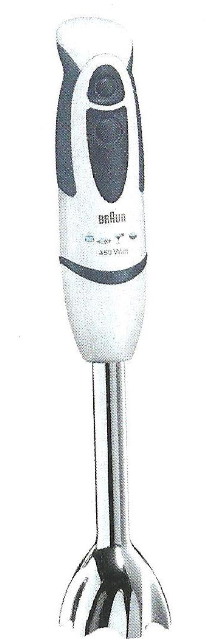
\includegraphics[width=1cm]{braum-mixer} 
        \caption*{Ganador del concurso de batidoras indesmontables... Braum y Kenwood!}
    \end{minipage}
    \hfill
    \begin{minipage}[b]{0.4\textwidth}
        \centering
        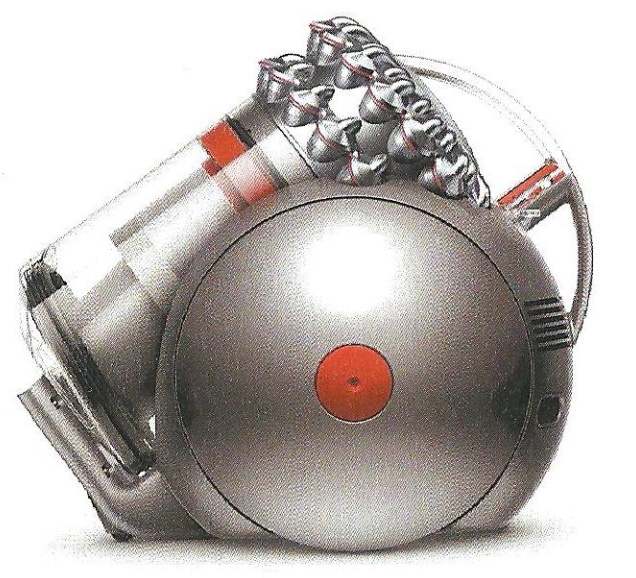
\includegraphics[width=2cm]{Dyson} 
        \caption*{¿Es para aspirar polvo intergaláctico?}
    \end{minipage}
\end{figure}



\end{itemize}


\chapter{Las bases de la electricidad}
\section{¿Qué es la electricidad?}
Con un poco de teoría, voy a explicar algunos conceptos básicos
para que entiendas lo que es la electricidad.
Así podrás medir y probar muchos de los componentes de tus
en tus electrodomésticos.

\begin{figure}[h]
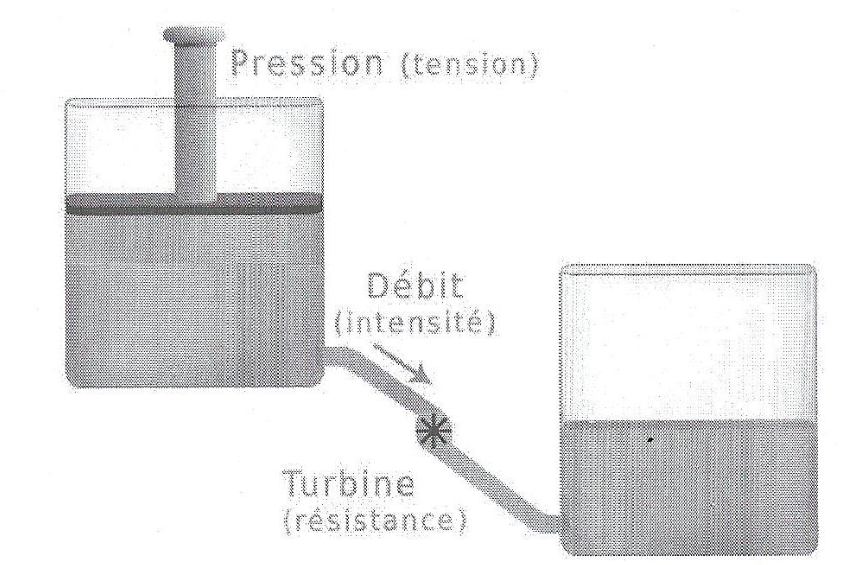
\includegraphics[width=0.8\textwidth]{analogia-agua-elec} 
\caption*{Analogía entre la electricidad y el agua}
\end{figure}

\begin{itemize}
\item \textbf{La tensión (U)} se expresa en voltios (V). Puede ser \textbf{Contínua}, como en una batería, salida del cargador, etc.) o \textbf{Alterna} (señales de la red eléctrica
señales electrónicas, etc.). Es una diferencia de potencial eléctrico entre dos
dos puntos. Siempre medimos una tensión entre dos puntos. Veremos más tarde cómo hacerlo. La tensión de una batería puede ser de 1.5V, 3V, 9V, la tensión de red ronda actualmente los 230V.

\item \textbf{La intensidad (I)} (o "corriente") se expresa en amperios (A).
Flujo de electrones a través de un hilo conductor con una determinada impresión.
A diferencia de la tensión, para que exista una corriente debe consumirse energía.
debe consumirse energía. ë
No hay corriente medible en una pila que no está conectada a nada.
- En este caso, decimos que no tiene "carga" (lo que no significa que no esté cargada en el sentido de que no esté conectada a nada).
 que no esté cargada en el sentido de una pila descargada, significa que
que no está suministrando energía).

\item \textbf{La resistencia (R)} se expresa en ohmios $\Omega$. Es muy baja
(a menudo se considera nula) para los metales y muy alta para el aire
el aire, el plástico o la madera seca, por ejemplo.
Por tanto, un cable eléctrico tendrá una resistencia muy cercana a 0$\Omega$ y el aire tendrá
una resistencia considerada infinita.
Algunos componentes electrónicos o elementos eléctricos también se denominan "resistencias"
o elementos eléctricos (por ejemplo, la resistencia de un horno eléctrico
horno o tostadora).
También existen resistencias "variables", ya sea por acción mecánica o por un cambio de temperatura.
o por un cambio de temperatura, por ejemplo.

\end{itemize}

\noindent\fbox{%
    \parbox{\textwidth}{%
La relación entre estos tres valores es $U(V) = R(\Omega) \times I(A)$, lo que implica que para una tensión fija, si disminuye la resistencia, la intensidad aumenta, y vice versa. Esto se comprende bien gracias al esquema de analogía entre el agua y la electricidad!
    }%
}\\

Para medir estos tres valores eléctricos, necesitamos una herramienta especial llamada "multímetro". (véase el capítulo 2.4).

\begin{figure}[h]
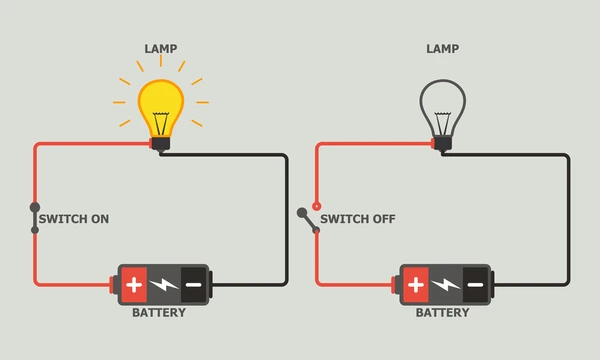
\includegraphics[width=0.7\textwidth]{circuito-abierto-cerrado} 
\centering
\caption*{Circuito abierto o cerrado (cambiar por otra figura)}
\end{figure}

\begin{enumerate}
\item Interruptor cerrado: la tensión "U" es igual a la tensión del generador, y ésta se extiende hasta los contactos de la lámpara (la tension en los extemos de un cable o de un interruptor cerrado siempre es de 0V). La corriente (I) existe y proporciona corriente a la lámpara para encenderse.
\item Interruptor abierto: la tensión "U" es igual a la tensión del generador, La tensión en los contactos de la lámpara es de 0V, no circula corriente
\end{enumerate}
La analogía con el agua no funciona aquí: un circuito cerrado significa que la electricidad puede circular.
posible circulación de electricidad, mientras que un grifo cerrado significa que no hay
circulación de agua...

\section{Los dispositivos de seguridad eléctrica}

\begin{large}
\textbf{a) Hilos y colores}\\
\end{large}
En primer lugar, para orientarse más fácilmente, hay que saber a qué corresponden los
corresponden en electricidad,
Pero como estos colores no siempre se respetan, veremos más adelante cómo estar seguros.
\begin{enumerate}
\item Para una tensión contínua:
\begin{itemize}
\item El hilo negro será el \textbf{-} (O a menudo el conector exterior en cables blindados)
\item El hilo rojo será el \textbf{+} (O a menudo el hilo conductor interior en cables blindados)
\end{itemize}


\begin{normalize}
Un cable "blindado" es un cable que está envuelto en un blindaje metálico conectado a la masa del aparato, para evitar interferencias electromagnéticas.
\end{normalize}

\item En lo que incumbe a instalaciones eléctricas: no se deje engañar por la posición del neutro y lugar del neutro y la fase en una toma eléctrica, esta norma no siempre se
esta norma no siempre se respeta, ya que si invierte el neutro y la fase, también
también funcionará.

\begin{figure}[h]
    \centering
    \begin{minipage}[b]{0.45\textwidth}
        \centering
        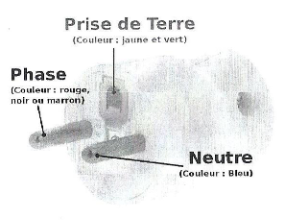
\includegraphics[width=\textwidth]{enchufe-macho} 
    \end{minipage}
    \hfill
    \begin{minipage}[b]{0.45\textwidth}
        \centering
        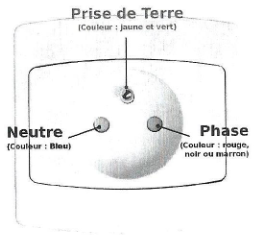
\includegraphics[width=\textwidth]{enchufe-hembra} 
    \end{minipage}
\end{figure}

\begin{itemize}
\item La fase (llegada de la corriente): todos los colores excepto azul y verde/amarillo. Puede estar directamente conectada al tablero de fusibles, o conecetada a un interruptor, por ejemplo
\item El neutro (escape de la corriente): azul
\item La tierra: verde y amarillo
\end{itemize}

\end{enumerate}

\newpage
\textbf{b) ¿De qué sirve la tierra y el disyunctor diferencial?}\\
Es importante comprender la finalidad de estos dos elementos, que han sido
creados para reducir el riesgo de electrocución de las personas en caso de avería de un aparato, como una fuga de agua en una lavadora, por ejemplo (el agua es un buen conductor de la electricidad)

\begin{figure}[h]
\includegraphics[width=0.7\textwidth]{diferencial-protección-tierra} 
\centering
\caption*{\textit{Los diferentes grados de protección de una instalación eléctrica}}
\end{figure}

Imagine un contacto eléctrico entre un cable conectado a un potencial eléctrico peligroso
(como la red de 230 V) y la carcasa metálica de su frigorífico.
de su frigorífico.

\begin{itemize}
\item Caso de la primera imagen: sin tierra ni disyunctor diferencial.
Si un apersona toca el frigorífico, la corriente pasará por el cuerpo de ésta para retornar a la tierra (ya que la corriente de la red está referenciada a tierra y siempre busca volver a ella, un poco como si se sintiese atraída por ella).

\textbf{$\Rightarrow$ La persona se electrocuta}

\item Caso de la segunda imagen: el cable de tierra está presente, es decir
todas las partes metálicas de los aparatos eléctricos están conectadas eléctricamente a tierra, pero sigue sin haber interruptor diferencial.
Esta vez, si alguien toca el frigorífico, la corriente fluirá a través del cable de tierra Y a través del cuerpo de la persona.

\textbf{$\Rightarrow$ La persona se da un calambre}
\newpage

\begin{normalize}
La corriente será mucho menor en el cuerpo de la persona que en el cable de tierra, porque la resistencia eléctrica entre la mano y los pies de una persona es mucho mayor que la de un cable de cobre. Cuanto menor sea esta resistencia (dedos y pies mojados, sobre un suelo húmedo, etc.), mayor será la fuga a tierra. Más fuerte y, por tanto, más peligrosa será la corriente.
\end{normalize}

\item Último caso: incluso antes de que alguien toque el aparato averiado, el disyuntor diferencial detectará la fuga de corriente y cortará la corriente a toda la instalación eléctrica. Se trata de la famosa palanca o botón grande que suele colocarse junto al contador de la luz.

\end{itemize}

\begin{figure}[h]
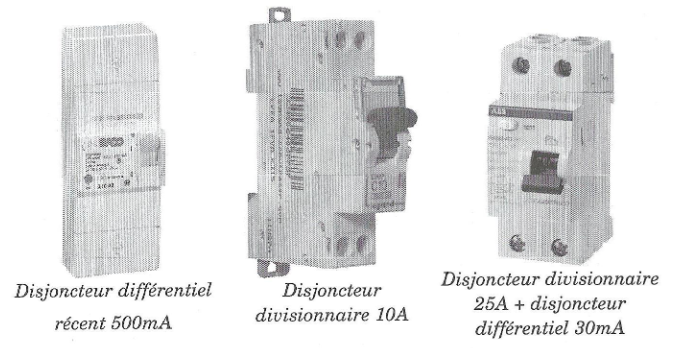
\includegraphics[width=0.9\textwidth]{disyunctores} 
\centering
\end{figure}

El interruptor diferencial mide la corriente que entra en la vivienda a través de la fase y la corriente que sale de la vivienda a través del conductor neutro.
Si la diferencia supera los 500 mA (650 mA en los modelos más antiguos), se dispara.
En ese caso, suele significar que un aparato conectado (no necesariamente en funcionamiento) está averiado.
Los interruptores diferenciales no deben confundirse con los interruptores divisionales.
disyuntores, que ahora sustituyen a los antiguos fusibles.\\

La función de un disyuntor divisor es cortar la electricidad a una parte de la instalación cuando se produce una sobreintensidad en dicha parte, es decir, cuando se produce un sobreconsumo anormal de corriente.
Generalmente, se disparan a los 16A para los enchufes convencionales, a los 10A
para el alumbrado (también los hay de 20A o 32A para alimentar determinados aparatos de alto consumo: cocina eléctrica, termo...).

La causa de esta sobreintensidad puede ser un aparato defectuoso, pero también puede ser el consumo normal de varios aparatos conectados al mismo circuito.
ser el consumo normal de varios aparatos conectados al mismo circuito de
circuito (no necesariamente el mismo enchufe).

\noindent\fbox{%
    \parbox{\textwidth}{%
Ejemplo: un termo eléctrico con una potencia P de 2300W, consumirá una corriente de 10A ($P = U \times I \rightarrow I = P/U = 2300W / 230V = 10A$)
Si enchufais uno o más aparatos sobre el mismo circuito, cuyo consumo sobrepase 6A, el disyunctor divisionario o el fusible de 16A cortará el circuito: $10+6=16A$
    }%
}\\

En las instalaciones recientes, se montan en el mismo módulo un disyuntor y un interruptor diferencial para cada parte de la instalación. Estos disyuntores diferenciales suelen dispararse a 30mA y por una buena razón:

\begin{figure}[h]
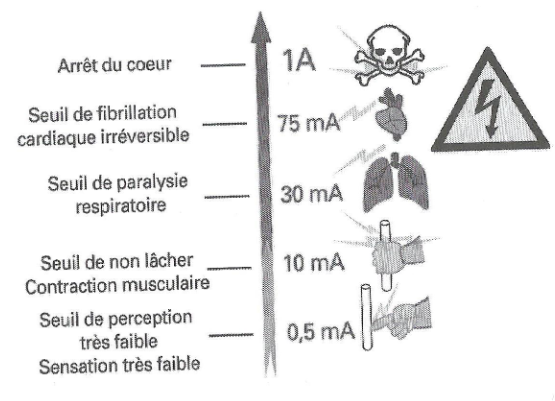
\includegraphics[width=0.9\textwidth]{corriente-efectos} 
\centering
\end{figure}

\textbf{b) ¿Cómo verificar una buena conexión a tierra?}\\
El disyunctor diferencial, está presente hoy en día en la mayor parte de instalaciones eléctricas de España, mientras que la toma de tierra está desgraciadamente ausente en muchas (la presencia de contactos de tierra en el enchufe no implica que esté conectada) Hay que coger el hábito de verificar si la tierra está bien conectada a los enchufes que vamos a usar para nuestros aparatos (sobre todo si hay facilidad de contacto con partes metálicas) Para ello, utilizaremos el multímetro (ver capítulo 2.4) en modo voltímetro en un rango de alterna superior a 240V.
\begin{itemize}
\item Entre el neutro y la fase deberíamos obtener 230V
\item Entre la fase y la tierra igualmente 230V (si no: tierra mal conectada)
\item Entre el neutro y la tierra, no más de 5V (si no: tierra mal conectada)
\end{itemize}
\newpage

Estas mediciones también permiten determinar la ubicación de la fase y el neutro, que no siempre están colocados como se muestra en el diagrama siguiente:

\begin{figure}[h]
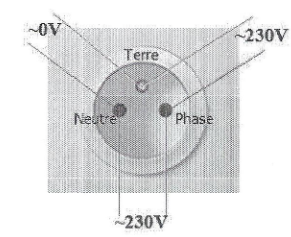
\includegraphics[width=0.4\textwidth]{diagrama-enchufe} 
\centering
\end{figure}
\section{Los peligros eléctricos que podeis encontrar durante las reparaciones}
Si no sabes lo que haces, la electricidad puede ser peligrosa e incluso mortal.
Al solucionar problemas, intentamos evitar trabajar bajo tensión en la medida de lo posible, pero el peligro no siempre se elimina. Me refiero a la tensión de red, los 230V AC. Sin embargo, un dispositivo alimentado por una batería también puede ser peligroso.\\

\textbf{a) Aparato bajo tensión}\\

Como norma general, conecte un aparato a la red sólo para una prueba o medición rápida y desconéctelo inmediatamente después.

\begin{itemize}
\item En caso de medir con el aparato bajo tensión, hay que poner especial atención a no poner los dedos, o cualquier parte del cuerpo en contacto con el aparato, las manos deben de estar sobre las dos puntas del multímetro y lo más alejadas posible de la parte bajo tensión.
\item No se debe tener ningún recipiente con agua u otro líquido a proximidad del aparato y la mesa de trabajo debe estar despejada y limpia.
\item Intentad estar lo más aislado posible del suelo, con buenos zapatos de goma e idealmente una tabla de madera debajo.
\end{itemize}
\newpage

\textbf{b) Aparato sin tensión o alimentado por una pila/batería}\\
Aunque el aparato esté desenchufado, debe tener especial cuidado con
un componente electrónico fácilmente reconocible: el condensador.
\begin{figure}[h]
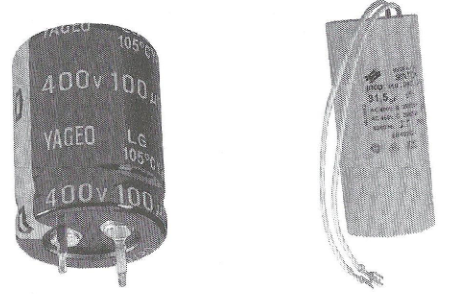
\includegraphics[width=0.7\textwidth]{condensadores} 
\centering
\end{figure}

Estos pequeños cilindros son capaces de almacenar alta tensión, lo que puede ser
peligroso.
Encontrará el modelo de la izquierda soldado a las tarjetas de alimentación de la mayoría de los aparatos más recientes conectados a la red que necesitan tensiones continuas. Pero también lo encontrarás en las cámaras digitales para dar al flash la potencia que necesita. El condensador de la derecha se encuentra en electrodomésticos como las lavadoras. También encontrará un condensador capaz de almacenar una tensión de unos 4000V en los hornos microondas: ¡una alta tensión muy peligrosa!
En ambos casos, la única forma de saber si debe desconfiar es
comprobar la tensión máxima admisible impresa en el componente.
Si supera los 50 V, deberá tomar las precauciones indicadas en el apartado
sección sobre condensadores (véase el capítulo 5.4.2).\\

En resumen, recuerde que los dispositivos potencialmente peligrosos, aunque estén apagados, son :
\begin{itemize}
\item Todos los aparatos alimentados por la red eléctrica equipados con una fuente de alimentación conmutada (véase el cap. 5.3.a)
\item Cámaras digitales
\item Hornos microondas
\item Tubos de rayos catódicos de pantallas y televisores antiguos
\end{itemize}


\end{document}
